\documentclass[12pt]{article}
\usepackage[margin=1in]{geometry}
\usepackage{amsmath,amssymb}
\usepackage{booktabs}
\usepackage{graphicx}
\usepackage{float}
\usepackage{enumitem}
\setlength{\parindent}{0pt}
\setlength{\parskip}{6pt}

\begin{document}

\begin{center}
    {\large Hayden Leung \\ Giacomo Cappelletto \\ \textbf{PY211 Lab 4 --- Projectile Motion}}
\end{center}

\section*{Objective}
Determine the initial velocity $v_0$ of a steel ball launched horizontally from a spring gun and study the dependence of the projectile range $R$ on the launch angle $\theta$.

\section*{Equipment}
\begin{itemize}[nosep]
    \item Spring gun with adjustable angle
    \item Steel ball
    \item Bar level
    \item Meter sticks
    \item Masking tape
    \item Paper (for marking landing positions)
\end{itemize}

\section*{Setup}
The spring gun was clamped to the edge of a table at a measured height $h$ above the floor. The angle of the gun could be adjusted using the built-in protractor, which reads the angle from the vertical. A sheet of paper was taped to the floor in the expected landing zone to record where the ball struck. The landing position was marked after each shot and its distance from the point directly below the launch point was measured with a meter stick to obtain the range $R$.

\section*{Process}
\begin{enumerate}[nosep]
    \item Set the spring gun to $\theta_{\mathrm{in}} = 0^\circ$ from vertical (horizontal launch) and measure the height $h$ from the center of the ball to the floor.
    \item Fire the ball 5 times, recording the range $R$ for each shot.
    \item Compute the mean range $\overline{R}$, its standard deviation $s_R$, and the standard error of the mean $\delta\overline{R} = s_R / \sqrt{n}$.
    \item Use $\overline{R}$ and $h$ to calculate the initial velocity $v_0$.
    \item Adjust the spring gun to angles of $10^\circ$, $15^\circ$, $20^\circ$, $25^\circ$, $30^\circ$, and $35^\circ$ from vertical. At each angle, measure $h$ and fire the ball 3 times, recording the range each time.
    \item For each angle, compute the measured mean range and its uncertainty, the calculated range $R_{\mathrm{calc}}$ from the theoretical equation, and the propagated uncertainty $\delta R_{\mathrm{calc}}$.
    \item Compare measured and calculated ranges using residuals and $z$-scores.
\end{enumerate}

\section*{Theory}

For a horizontal launch ($\theta = 0^\circ$ from horizontal), the initial velocity is:
\[
    v_0 = \overline{R}\,\sqrt{\frac{g}{2h}}
\]
where $g = 9.81\;\mathrm{m/s^2}$ is the gravitational acceleration and $h$ is the launch height.

The uncertainty on $v_0$ is obtained by error propagation:
\[
    \delta v_0 = v_0 \sqrt{\left(\frac{\delta\overline{R}}{\overline{R}}\right)^2 + \frac{1}{4}\left(\frac{\delta h}{h}\right)^2}
\]

For a launch at angle $\theta$ from the horizontal (where $\theta = 90^\circ - \theta_{\mathrm{in}}$ and $\theta_{\mathrm{in}}$ is the angle read from the apparatus, measured from vertical), the theoretical range is:
\[
    R_{\mathrm{calc}} = \frac{v_0^2 \cos\theta}{g}\left(\sin\theta + \sqrt{\sin^2\theta + \frac{2gh}{v_0^2}}\right)
\]

The uncertainty on $R_{\mathrm{calc}}$ is propagated from the uncertainties on $v_0$, $h$, and $\theta$:
\[
    \delta R_{\mathrm{calc}} = \sqrt{\left(\frac{\partial R}{\partial v_0}\,\delta v_0\right)^2 + \left(\frac{\partial R}{\partial h}\,\delta h\right)^2 + \left(\frac{\partial R}{\partial \theta}\,\delta \theta\right)^2}
\]

where the partial derivatives were evaluated numerically.

\section*{Assumptions}
\begin{itemize}[nosep]
    \item The gravitational acceleration is $g = 9.81\;\mathrm{m/s^2}$.
    \item Air resistance is negligible.
    \item The initial velocity $v_0$ is the same for every shot regardless of the launch angle (the spring compression is constant).
    \item The protractor on the apparatus reads the angle from the vertical accurately to within $\pm 0.5^\circ$.
    \item The ball behaves as a point mass launched from a single well-defined point.
\end{itemize}

\section*{Sources of Experimental Uncertainty \& Steps to Minimize}
\begin{itemize}[nosep]
    \item Variation in spring release from shot to shot $\rightarrow$ practiced firing the gun consistently before recording data; took multiple shots at each angle.
    \item Difficulty reading the exact landing position $\rightarrow$ placed paper on the floor and marked each impact point; measured from a consistent reference line directly below the launch point.
    \item Uncertainty in height measurement ($\delta h = 0.005\;\mathrm{m}$) $\rightarrow$ measured $h$ carefully with a meter stick at each angle setting, since tilting the gun changes the height of the ball's center.
    \item Uncertainty in angle reading ($\delta\theta = 0.5^\circ$) $\rightarrow$ used the bar level to verify the table was level; read the protractor scale as precisely as possible.
\end{itemize}

\section*{Results of Experiment}

\subsection*{Table 1: Calibration at $\theta_{\mathrm{in}} = 0^\circ$ (horizontal launch)}

\begin{table}[H]
\centering
\begin{tabular}{ccccccc}
\toprule
$\theta\;(^\circ)$ & $h\;(\mathrm{m})$ & $n$ & $\overline{R}_{\mathrm{meas}}\;(\mathrm{m})$ & $\delta\overline{R}\;(\mathrm{m})$ & $v_0\;(\mathrm{m/s})$ & $\delta v_0\;(\mathrm{m/s})$ \\
\midrule
0 & 1.015 & 5 & 1.816 & 0.0103 & 3.992 & 0.0247 \\
\bottomrule
\end{tabular}
\end{table}

Raw range measurements at $\theta = 0^\circ$: 1.84, 1.83, 1.81, 1.78, 1.82~m.

\subsection*{Table 2: Range vs.\ angle}

\begin{table}[H]
\centering
\small
\begin{tabular}{cccccccc}
\toprule
$\theta_{\mathrm{in}}\;(^\circ)$ & $\theta_{\mathrm{h}}\;(^\circ)$ & $h\;(\mathrm{m})$ & $\overline{R}_{\mathrm{meas}}\;(\mathrm{m})$ & $\delta\overline{R}\;(\mathrm{m})$ & $R_{\mathrm{calc}}\;(\mathrm{m})$ & $\delta R_{\mathrm{calc}}\;(\mathrm{m})$ & $z$ \\
\midrule
10 & 80 & 1.035 & 2.010 & 0.0029 & 0.700 & 0.0347 & 37.6 \\
15 & 75 & 1.040 & 2.068 & 0.0044 & 1.032 & 0.0337 & 30.5 \\
20 & 70 & 1.050 & 2.190 & 0.0076 & 1.342 & 0.0325 & 25.4 \\
25 & 65 & 1.070 & 2.288 & 0.0093 & 1.626 & 0.0310 & 20.5 \\
30 & 60 & 1.080 & 2.330 & 0.0058 & 1.875 & 0.0293 & 15.2 \\
35 & 55 & 1.090 & 2.343 & 0.0067 & 2.085 & 0.0277 & 9.07 \\
\bottomrule
\end{tabular}
\end{table}

Here $\theta_{\mathrm{in}}$ is the angle from vertical read on the apparatus, $\theta_{\mathrm{h}} = 90^\circ - \theta_{\mathrm{in}}$ is the angle from horizontal used in the range equation, and $z = (\overline{R}_{\mathrm{meas}} - R_{\mathrm{calc}}) / \sqrt{(\delta\overline{R})^2 + (\delta R_{\mathrm{calc}})^2}$ is the $z$-score comparing the two.

\section*{Graphical Analysis}

\begin{figure}[H]
    \centering
    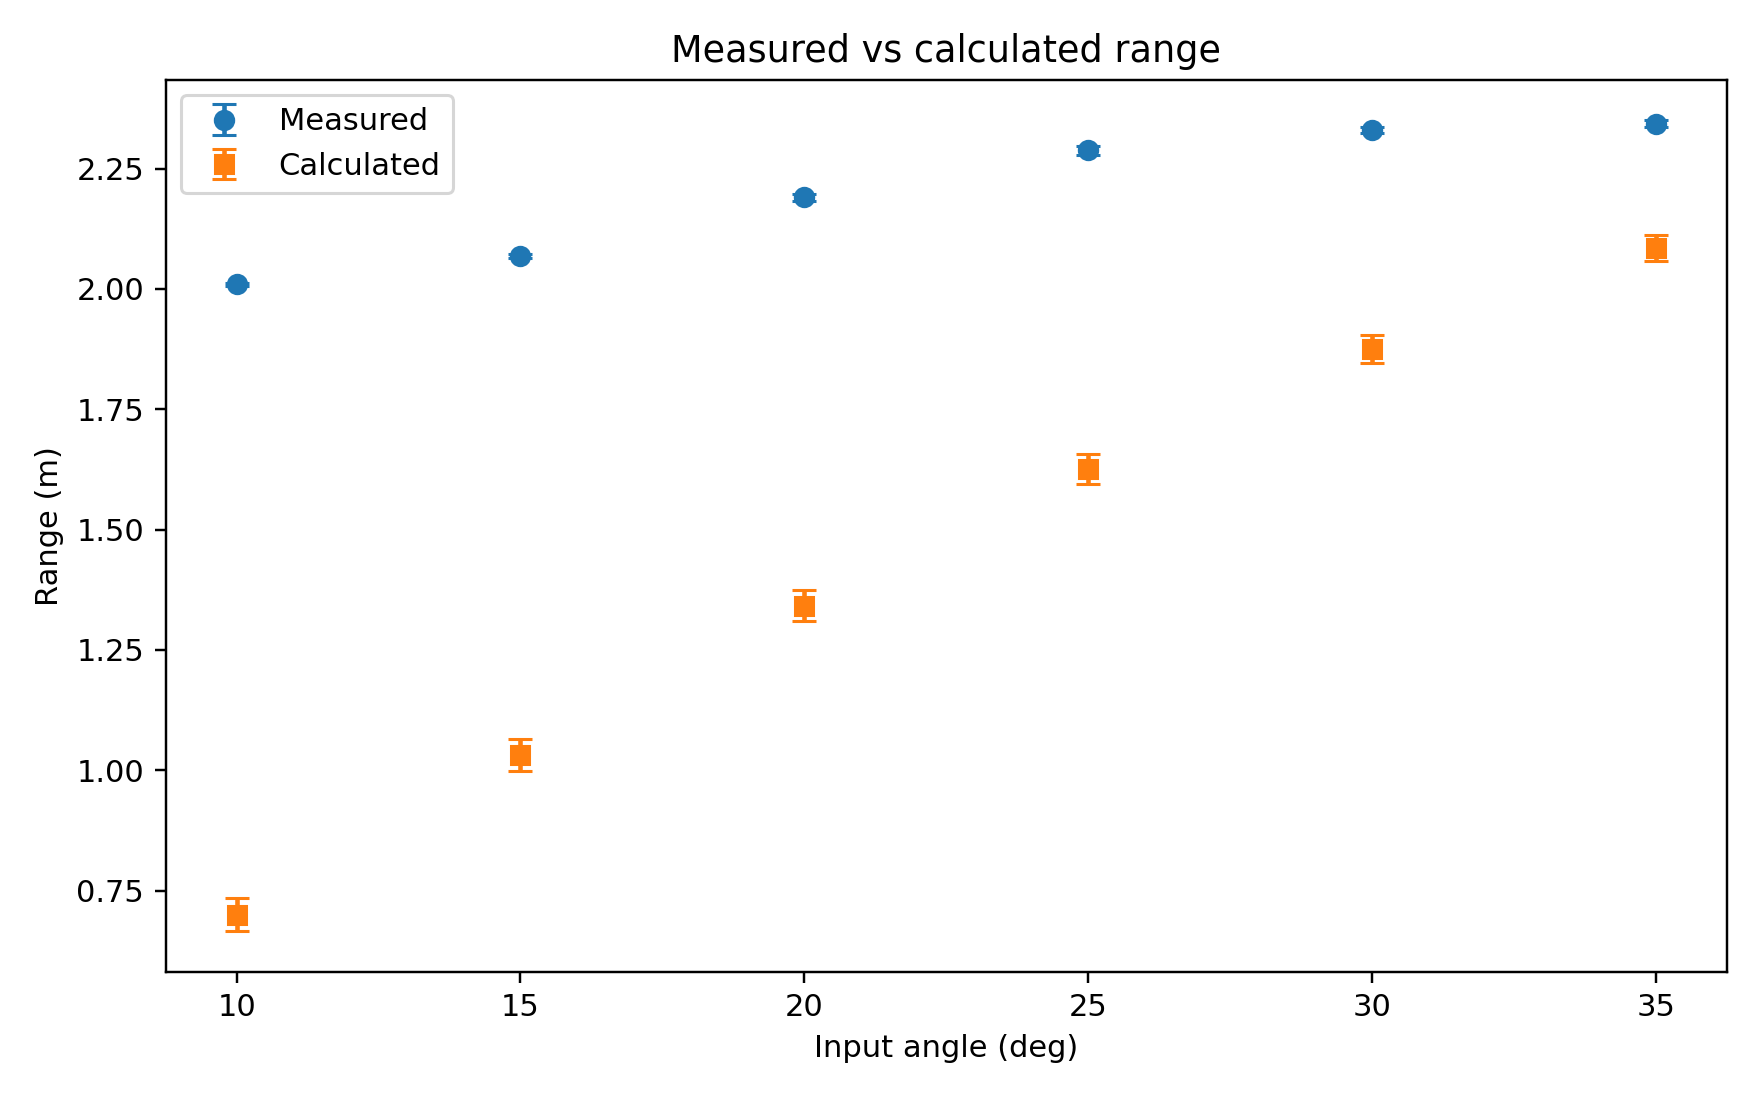
\includegraphics[width=0.75\textwidth]{projectile_lab_output/measured_vs_calculated_range.png}
    \caption{Measured and calculated range as a function of the input angle (from vertical). Error bars represent $\delta\overline{R}$ and $\delta R_{\mathrm{calc}}$ respectively.}
\end{figure}

\begin{figure}[H]
    \centering
    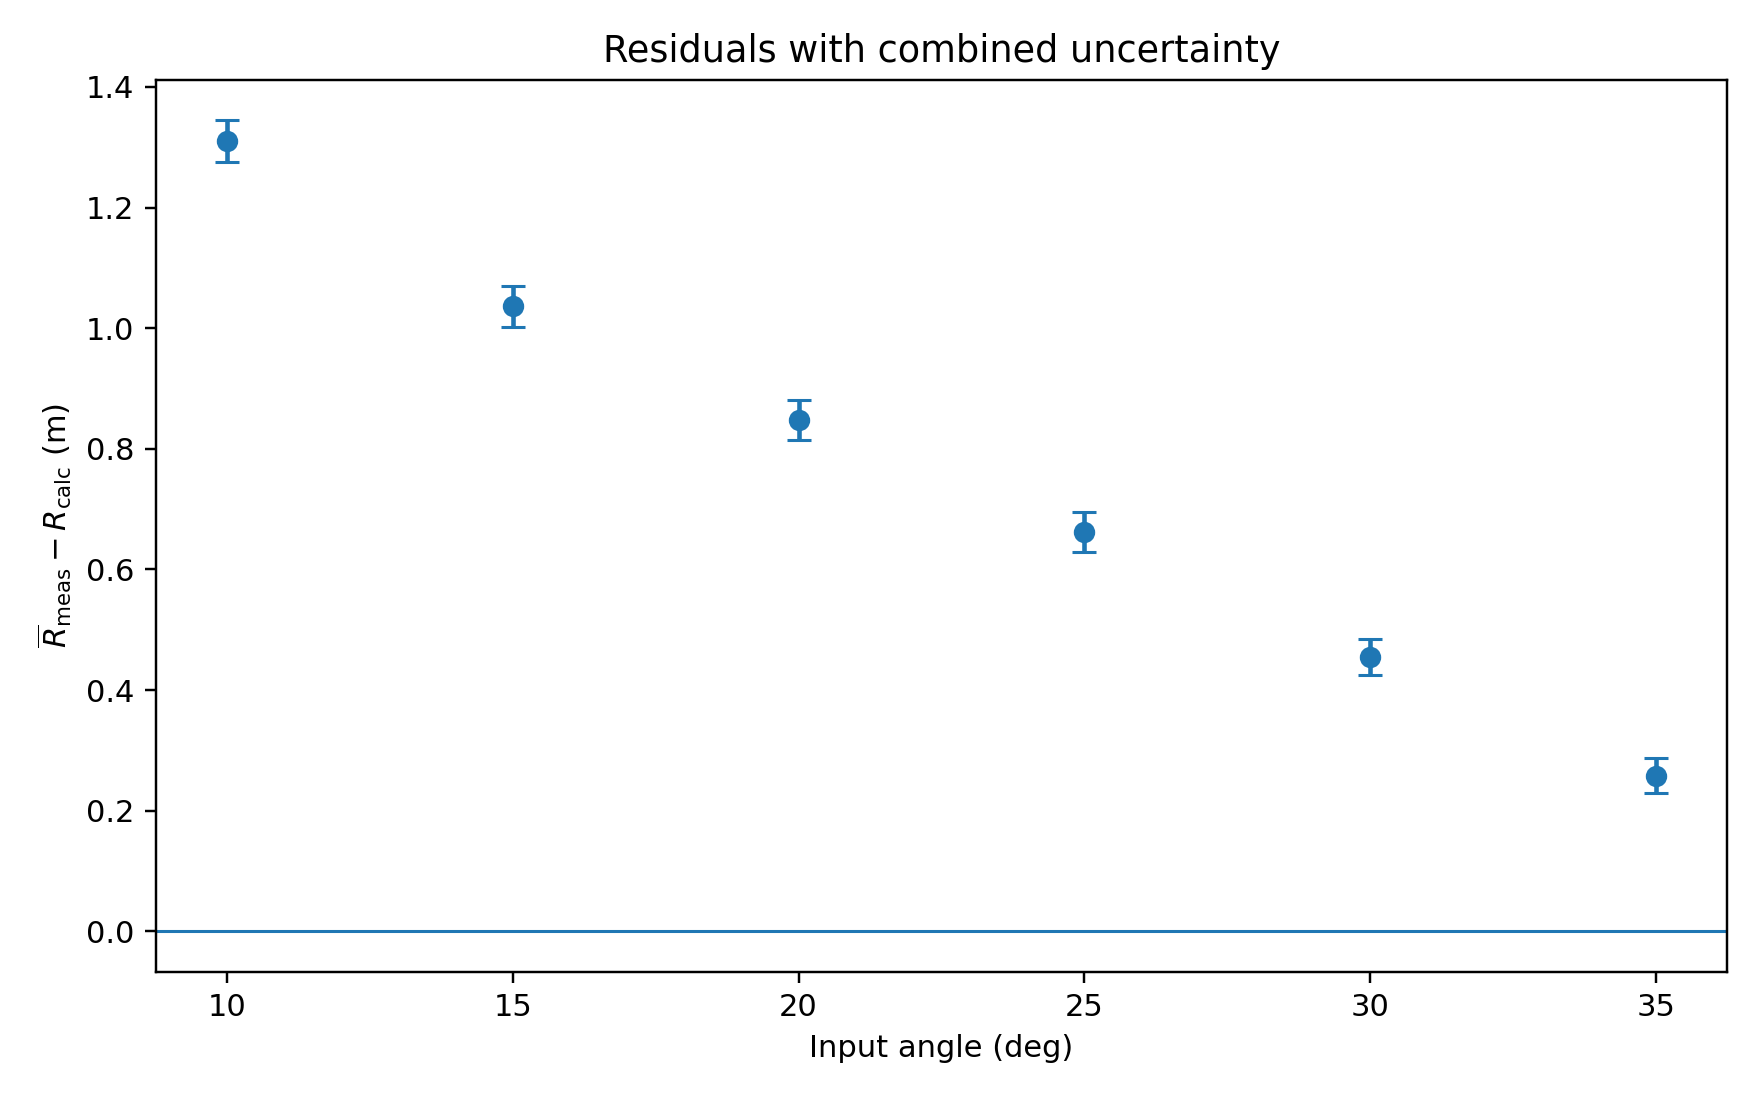
\includegraphics[width=0.75\textwidth]{projectile_lab_output/residuals_vs_angle.png}
    \caption{Residuals $(\overline{R}_{\mathrm{meas}} - R_{\mathrm{calc}})$ with combined uncertainty at each angle.}
\end{figure}

\begin{figure}[H]
    \centering
    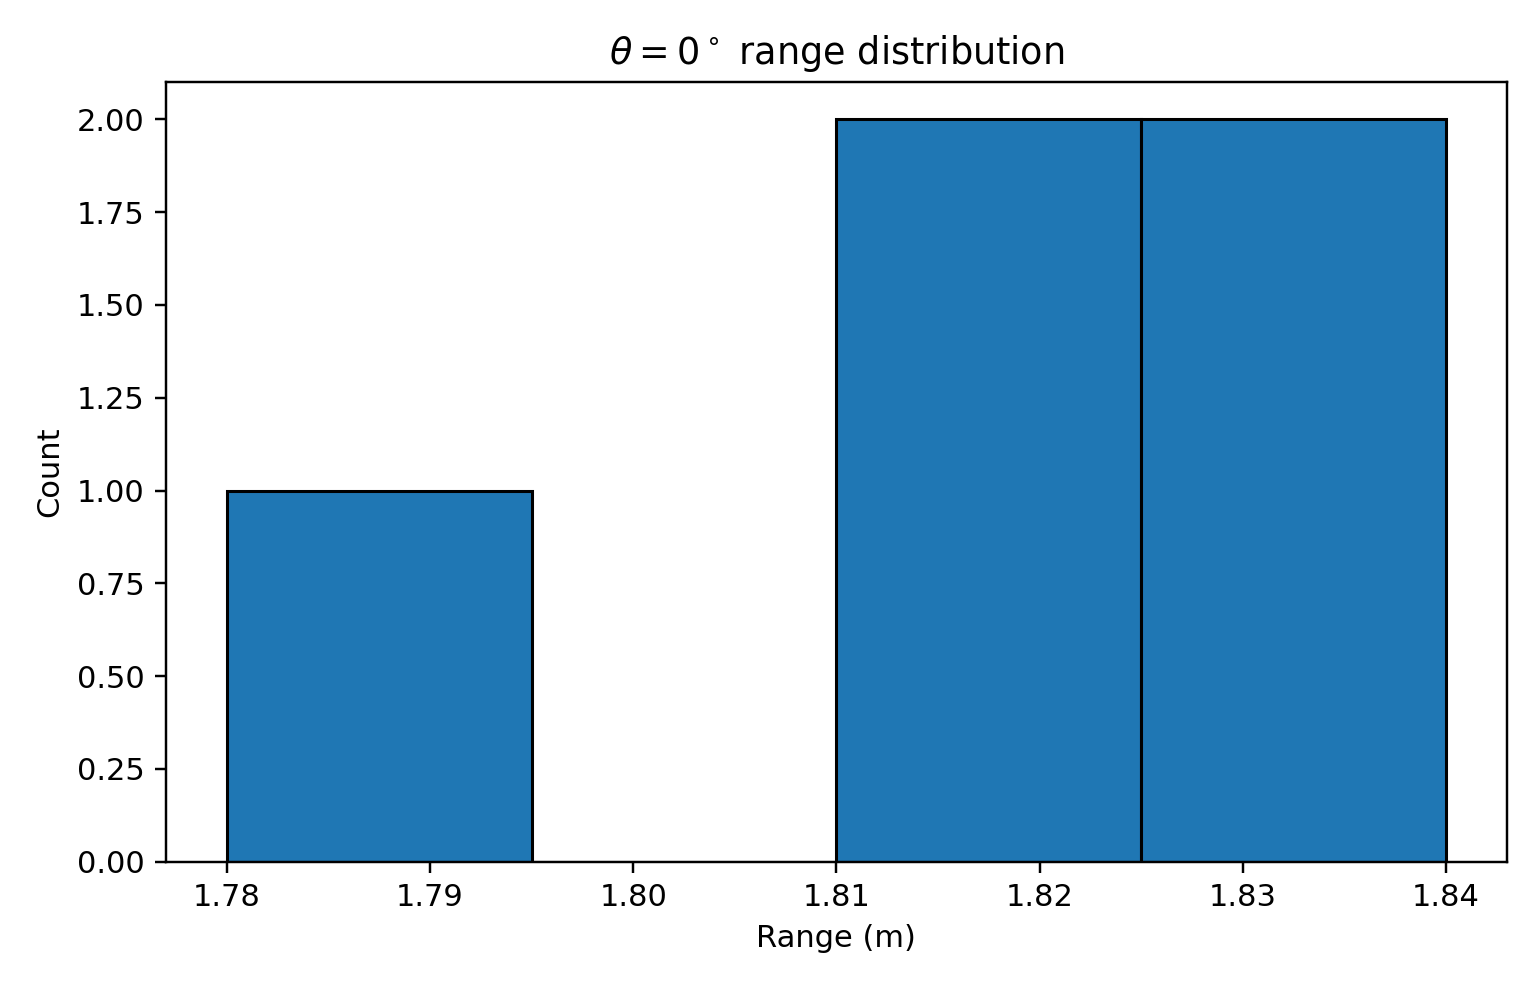
\includegraphics[width=0.55\textwidth]{projectile_lab_output/calibration_range_distribution.png}
    \caption{Distribution of the five range measurements at $\theta = 0^\circ$.}
\end{figure}

\section*{Calculations}

Detailed, step-by-step calculations with full substitutions and uncertainty propagation for every trial are provided in the attached document \texttt{projectile\_lab\_show\_work.pdf}.

As a representative example, the calibration velocity:
\[
    v_0 = (1.816)\sqrt{\frac{9.81}{2(1.015)}} = 3.992\;\mathrm{m/s}
\]
\[
    \delta v_0 = (3.992)\sqrt{\left(\frac{0.0103}{1.816}\right)^2 + \frac{1}{4}\left(\frac{0.005}{1.015}\right)^2} = 0.0247\;\mathrm{m/s}
\]

\section*{Conclusion}

The initial velocity of the steel ball was found to be $v_0 = (3.992 \pm 0.025)\;\mathrm{m/s}$. At all six angles ($10^\circ$--$35^\circ$ from vertical), the measured ranges exceeded the calculated values, yielding $z$-scores between 9 and 38---well above the consistency threshold of 2. The discrepancy shrinks as the gun approaches horizontal, suggesting a systematic effect tied to the tilt of the barrel, such as a change in effective launch height $h$ or reference point when the gun is angled. These effects are not reflected in our statistical uncertainties. The qualitative trend is nonetheless correct: range increases monotonically as the angle approaches horizontal, consistent with theory. More careful measurement of $h$ and the range reference at each angle setting would reduce the systematic offset.

\end{document}
